\chapter{Consequences of Relativity}
\section{Time Dilation and the Decay of Unstable Particles}
Unstable particle decay after a certain time, but by observing how long they take to decay when traveling at relativistic speeds we can observe the effects of time dilation. \\
Statistically according to the exponential-decay law 
\[ N ( t ) = N ( 0 ) e ^ { - t / \tau } \]
where $ N(t) $ is the number of particles present at time $ t $, given that $ N(0) $ is the number present at the initial time $ t = 0 $. \\
To an observer moving at relativistic velocity $ v $ in the $ x- $direction with respect to $ S $, time will be 
\[ t' = \gamma(v) t \]. If we consider the fraction
\[ N ( t ) / N(0) = e^{-t/\tau} \]
both $ t $ and $ \tau $ will be dilated, in other words
\[ \tau' = \gamma \tau \]
so the fraction of the particles remaining is the same as viewed by both the rest and moving observer. \\
We can see the effects of time dilation on the \textbf{muon} particle, $ \mu $. 
\begin{example}
	A beam of muons is injected in a storage ring, a device that uses electromagnetic fields to maintain the muons in uniform circular motion. The ring's radius is $ 60 $m, and the muons are injected with a velocity such that $ \gamma = 15 $. How many revolutions of the ring will an "average" muon make before it decays? The proper lifetime of a muon is $ 2.2 \times 10^{-6} $s. \\
	\textbf{Solution.} We can find the speed of the muons using $ \gamma $.
	\[ \frac { v } { c } = \sqrt { \frac { \gamma ^ { 2 } - 1 } { \gamma ^ { 2 } } } = \sqrt { \frac { 15 ^ { 2 } - 1 } { 15 ^ { 2 } } } = 0.998 \]
	and the distance it travels in its lifetime is 
	\begin{align*}
	x = y v \tau = 15 \times ( 0.998 ) \left( 3 \times 10 ^ { 8 } m / s \right) \\\left( 2.2 \times 10 ^ { - 6 } s \right) = 9.88 \times 10 ^ { 3 } \mathrm { m }
	\end{align*}
\end{example}
\section{Relativistic Doppler Shift}
We discussed this earlier with light, frequency and wavelength. \\
The frequency in the source's rest frame is called \textbf{proper frequency}. We know these are connected by
\[ \lambda = cT \]
Now consider the situation where the observer is moving with velocity $ v $ away from the source. First, the observer moved away a distance $ vT' $ and second the original distance $ \lambda $ will have Lorentz contracted to \[ \lambda\sqrt{1-v^2/c^2} \]
Putting this together the total distance the light would have traveled between pulses is 
\[ c T ^ { \prime } = v T ^ { \prime } + \lambda \sqrt { 1 - v ^ { 2 } / c ^ { 2 } } \]
replacing $ \lambda $ and solving for $ T' $
\[ T ^ { \prime } = T \sqrt { \frac { 1 + v / c } { 1 - v / c } } \]
Since frequency is the inverse of period
\[ f ^ { \prime } = f \sqrt { \frac { 1 - v / c } { 1 + v / c } } \]
\indent Now consider the source is in motion, and to observer is not. So, the distance the light travels, $ cT' $, is given by 
\[ c T ^ { \prime } = \gamma T \times ( c + v ) \]
which finally gives us
\[ c T ^ { \prime } = \gamma T ( c + v ) = c T \frac { 1 + v / c } { \sqrt { 1 - v ^ { 2 } / c ^ { 2 } } } = c T \sqrt { \frac { 1 + v / c } { 1 - v / c } } \]
\indent Imagine the use of this in \textit{Doppler Radar} that can not only tell us position through time delay but also frequency shift and give information about the objects motion!
\section{Mass, Momentum and Energy}
What happens when you try to go faster and faster to the speed of light? It gets harder to accelerate because, as
\[ v \rightarrow c, \gamma \rightarrow \infty \]
A weird thing to consider is that massless objects like photons do travel at the speed of light, and so may other massless objects. \\
The quick result for momentum with relativity is 
\[ \vec { \mathrm { p } } = \gamma m \vec { \mathrm { v } } \]
We know classically 
\[ W_{net} = \Delta KE  \]
thus we can simply find that 
\[ W_{net} = mc^2(\lambda - 1) \]
This derivation is a solution in the test for this chapter. \\
We can also find the energy by 
\[ E = \sqrt{p^2 c^2 + m^2c^4} \]
dropping mass for massless objects this becomes
\[ E = pc \]
\section{The Equivalence of Mass and Energy}
\section{Forces in Relativity}
The one equation we need is 
\[ F = \dfrac{dp}{dp} \]
where 
\[ p \equiv \gamma m v \]
A special case for \textbf{constant force}. Suppose that a constant force of magnitude $ F_0 $ acts in the x-direction, starting at $ t = 0 $, when the object is at rest. 
\[ F_0 = \dfrac{d}{dt} (\gamma(u)mu) \]
for the object's speed $ u $, where $ dx/dt = u $. Since $ F_0 $ is constant integrating with respect to $ t $ gives us 
\[ (F_0t)/m = \gamma(u) u + C \]
consider initial conditions, $ u = 0 $ and $ t = 0 $, then $ C = 0 $. Solving for $ u $ we get 
\[ u = \dfrac{(F_0t/m)}{\sqrt{1 + \dfrac{F_0^2t^2}{m^2c^2}}} \]
which has the property that sets the speed limit of $ c $. \\
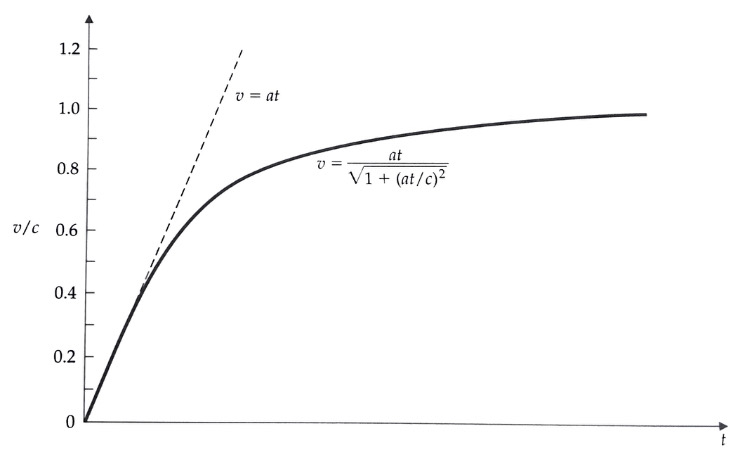
\includegraphics[width=\columnwidth]{constantforce}
\begin{example}
	Find the position of an object of mass $ m $ on which the constant force acts as a function of time. \\
	If we integrate
	\[ u = \dfrac{(F_0t/m)}{\sqrt{1 + \dfrac{F_0^2t^2}{m^2c^2}}} \]
	with respect to time, we will get position. Lets say $ x,t = 0 $ we get
	\[ x ( t ) = \frac { m c ^ { 2 } } { F _ { 0 } } \left( \sqrt { 1 + \frac { F _ { 0 } ^ { 2 } t ^ { 2 } } { m ^ { 2 } c ^ { 2 } } } - 1 \right) \]
	
\end{example}





